%----------------------------------------------------------------------------
\chapter{Megvalósítás}
%----------------------------------------------------------------------------
\section{Szükséges eszközök}
\subsection{Eclipse}
A feladat elkészítéséhez Eclipse-et használtam. Ez egy szabadon bővíthető nyílt forráskódú szoftverkeretrendszer. Eclipse-et a bele integrált fejlesztői környezetek segítségével nagyon sok mindenre lehet használni. Azért ezt választottam mert a modellezés általam használt részeihez is biztosít megfelelő keretrendszereket.
\subsection{EMF}
EMF az Eclipse Modelling Framework rövidítése. Ez egy olyan keretrendszer, mely az eclips-be beépülve teszi lehetővé modellek készítését. Segítségével könnyedén grafikus eszközökkel lehet metamodelleket alkotni, melyből később konkrét példánymodellt készíthetünk. Továbbá lehetőséget biztosít metamodellből java kódot generálni, ami leképezi a modell elemeit osztályokba és a hozzá tartozó kapcsolatokat és attribútumokat is.
\subsection{Java}
Objektum orientált programozási nyelv. Szerepe a kódgenerálásnál van. Az EMF modellből kigenerált kódot futtatva egy új Eclipse alkalmazás indítható, melyben már lehetőség van a metamodellben definiált modell példányosítására.
\subsection{Sirius}
Ez egy szintén Eclipse-be épülő keretrendszer. Ez lehetővé teszi hogy EMF modellekhez vizuális megjelenítő és szerkesztő felületet készítsünk. Rendkívül sokrétű lehetőséget nyújt. Lehetőség van új objektumok létrehozására szerkesztésére és biztosít validációs lehetőségeket is. Az egyes elemek módosítását megszorításokhoz lehet kötni. Egy úgynevezett "viewpoint specification" projektet kell létrehozni, majd ezen belül egy "odesign" kiterjesztésű fájlt. Ki kel választani milyen modellel szeretnénk dolgozni és azután lehet a modellhez tartozó editor működését és megjelenését definiálni.
\subsection{Aql}
Az Annotation Query Language rövidítése. Lamda kifejezésekhez hasonlóan lehet alkalmazni. Az editor elkészítésébe van nagy szerepe. Az egyes funkciókat előfeltételeit lehet leírni ezen a nyelve. 

\section{Metamodell szerkezete}

\subsection{Általános modell}

\subsubsection{Jellemzés}
Egy általános modell elemekből áll, amik tulajdonságokkal rendelkeznek, az elemek között pedig kapcsolatok vannak. Tehát olyan meta modellt kell készíteni, ami mindezeket magába foglalja. A metamodell elkészítéséhez EMF-et használtam.

\begin{figure}[!ht]
	\centering
	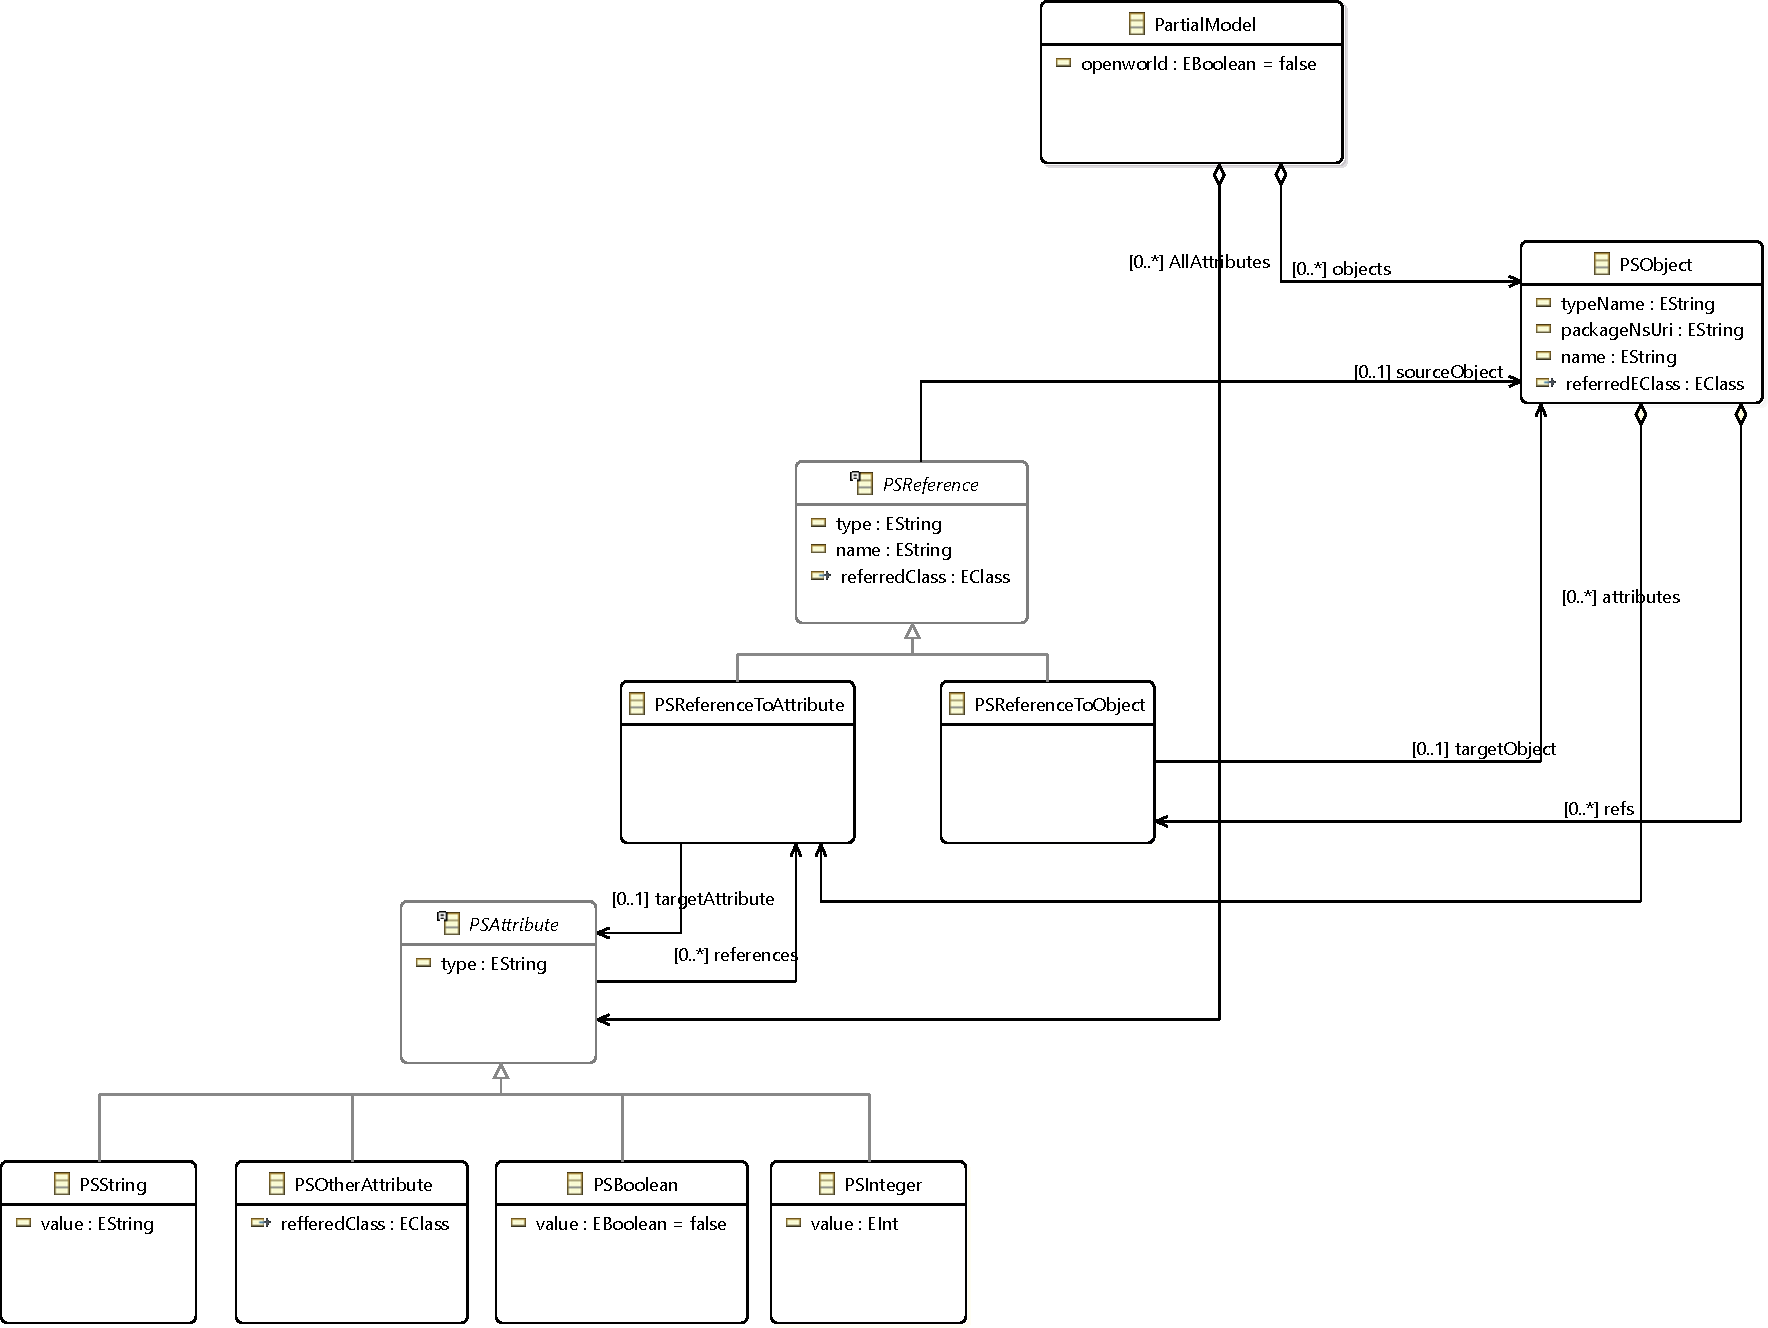
\includegraphics[width=150mm]{figures/partialmodel01.pdf}
	\caption{Általános modell, ami legtöbb modell metamodelljének tekinthető} 
\end{figure}

\subsubsection{PartialModel}
A fenti modellben a PSObject-ek reprezentálják az általános modell elemeit. Ez bármilyen típusú lehet. A PSObject attribútumokat (PSAttribute) tartalmaz, amik szintén bármilyen típusban és számosságban megjelenhetnek. 

\subsubsection{PSReference}
 Az elemek közötti kapcsolatokat reprezentálják. Fontos, hogy ezek is külön elemként jelenjenek meg a modellben, hisz ehhez is szeretnénk majd részlegességet társítani annotációk formájában. A PSReference egy absztrakt objektum két leszármazottja van a  PSReferenceToAttribute és PSReferenceToObject. Erre azért volt szükség mert későbbiekben a szerkesztő elkészítésénél más funkcionalitások vonatkoznak rájuk. 

\subsubsection{PSAttribute}
Az objektumok tulajdonságai külön egy PSAttribute nevű elemben vannak hozzárendelve az objektumokhoz, így lehetőség van az attribútumokhoz is részlegességet rendelni. Lehetséges továbbá az is hogy egy attribútum több objektumhoz is tartozzon, ugyanis az attribútumokat nem közvetlenül a PSObjeckt-ek tárolják hanem csak hivatkoznak rájuk. PSAttribute is absztrakt ezért több fajtája lehet:

\begin{itemize}  
	\item PSString
	\item PSBoolean
	\item PSInteger
	\item PSOtherAttribute 
\end{itemize}


\subsection{Kiegészítés részleges modellé}

\subsubsection{OW részlegesség}
Az \textit{OW} részlegességet a modell gyökerében egy boolean változóval tudjuk szemléltetni. Fenti metamodell alapján lehetőségünk van részleges modellek készítésére.

\subsubsection{PSType}
Minden egyes modellbeli elemhez tudnunk kell társítani annotációkat. Ezt a PSType-al tehetjük meg, amiből leszármaznak a már említett részlegesség fajták (\textit{May}, \textit{Var}, \textit{Abs}):

\begin{itemize}  
	\item MayType
	\item AbsType
	\item VarType 
\end{itemize}

\begin{figure}[!ht]
	\centering
	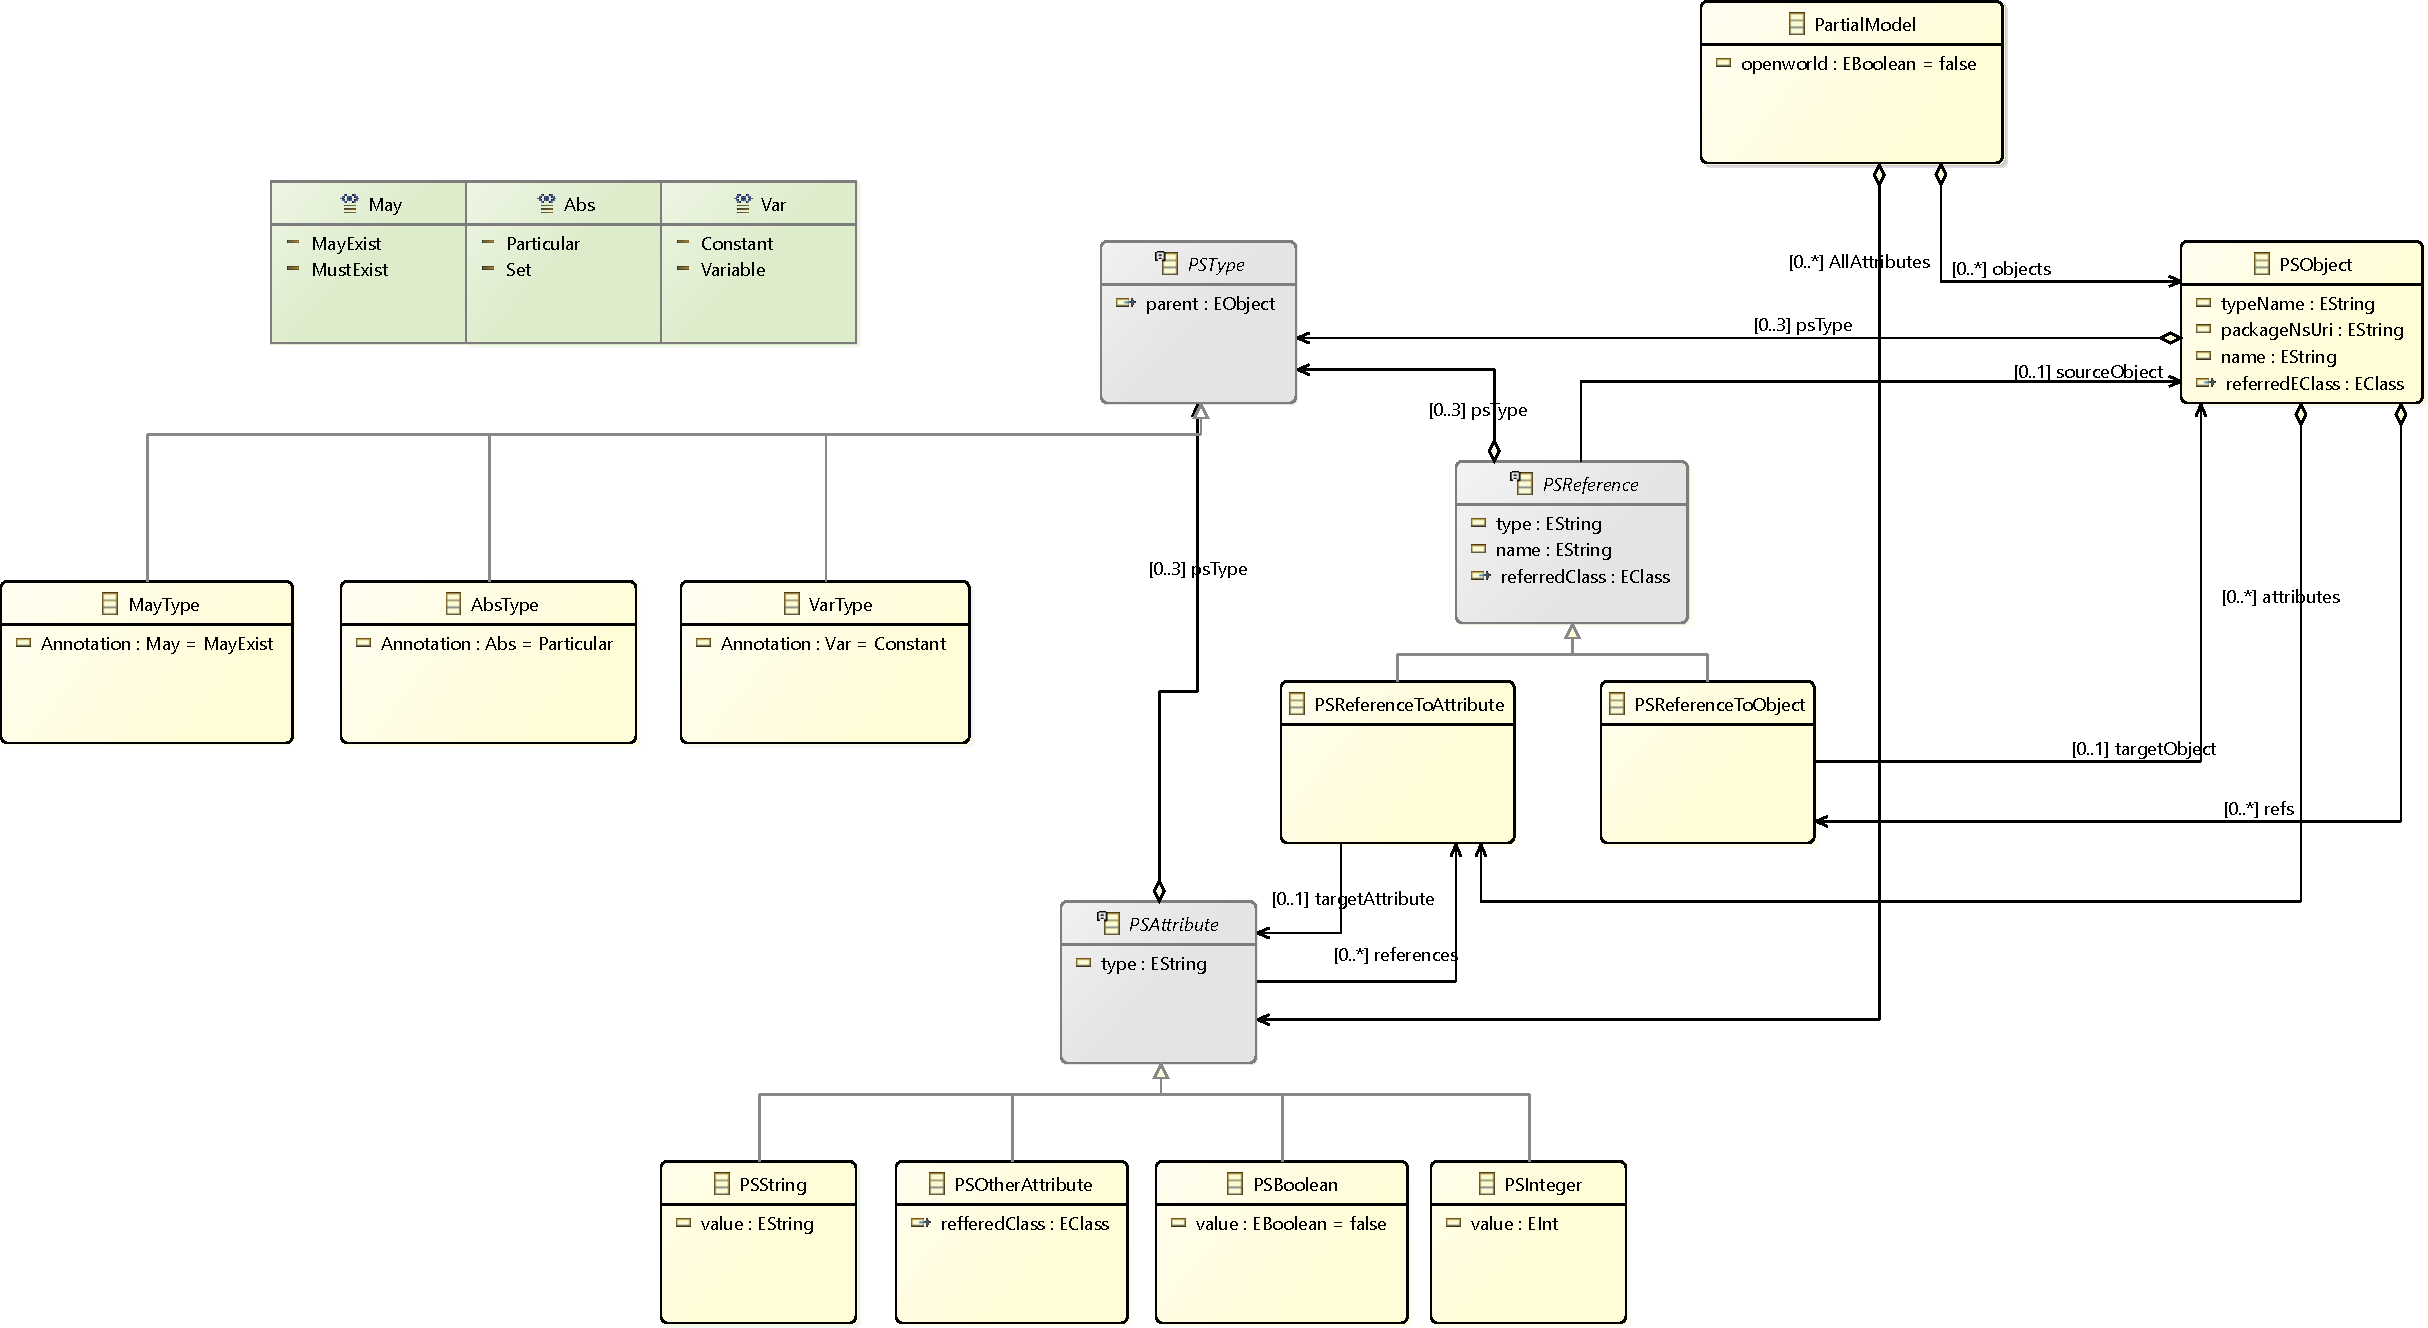
\includegraphics[width=150mm]{figures/partialmodel02.pdf}
	\caption{Általános modell kiegészítve részleges modellekre jellemző tulajdonságokkal} 
\end{figure}



\subsection{Példánymodell felülete}
Editort Sirius segítségével készítettem el. A PSObject-ek 
\subsection{Funkciók}